\documentclass[10pt,a4paper,titlepage]{report} 

% Include basis configuration
\usepackage[utf8]{inputenc}
\usepackage{usecases}
\usepackage{enumitem}
\usepackage{xparse}
\usepackage{array}
\usepackage{notes}
\usepackage[pdfpagelabels,pagebackref]{hyperref}
\usepackage[acronym,toc]{glossaries}
\usepackage{graphicx}
\usepackage[T1]{fontenc}
\usepackage{titlesec, blindtext, color}

\DeclareGraphicsExtensions{.pdf,.png}

% === Title page variables ===
% Authors
\newcommand \mehr{\Large\it Mehrdad Khodaverdi mehr@itu.dk}
\newcommand \siak{\Large\it Simon Alexander Kern siak@itu.dk}
\newcommand \tbch{\Large\it Thomas Bo Christiansen tbch@itu.dk}
\newcommand \ndom{\Large\it Nicklas Doolewerdt Mariager Johansen ndom@itu.dk}
\newcommand{\authors}{\Large\it \mehr \and \siak \and \tbch \and \ndom}
% System name
\newcommand \systemname{Glitter}
\newcommand \systemnamens{AutoSys}
% System version
\newcommand \systemversion{Version 1.0 }
% Company name
\newcommand \companyname{IT University of Copenhagen, Denmark}
% The date of the document
\newcommand \documentdate{\today}
% Legal references
\newcommand \legal[2]{\S#1 stk.\ #2}

\definecolor{Orange}{rgb}{1,0.5,0}
\definecolor{Blue}{rgb}{0,0,1}
\newcommand{\comment}[1]{\emph{\textcolor{Blue}{[#1]}}}
\newcommand{\todo}[1]{\textsf{\textbf{\textcolor{Orange}{[[#1]]}}}}

% === Glossaries ===
\makeglossaries
\renewcommand{\acronymname}{Definitions, acronyms, and abbreviations}
\renewcommand*{\glossarysection}[2][]{\ifnum\pdfstrcmp{#1}{Glossary}=0 \chapter{#1} \else \section{#1} \fi }
%\renewcommand*{\glspostdescription}{} % Remove the dot/period after the decription in the glossary.

\usepackage{acronym}

% Code (Java) listings
\usepackage{listings}
\usepackage{color}

\definecolor{dkgreen}{rgb}{0,0.6,0}
\definecolor{gray}{rgb}{0.5,0.5,0.5}
\definecolor{mauve}{rgb}{0.58,0,0.82}

\lstset{frame=tb,
  language=Java,
  aboveskip=3mm,
  belowskip=3mm,
  showstringspaces=false,
  columns=flexible,
  basicstyle={\small\ttfamily},
  numbers=none,
  numberstyle=\tiny\color{gray},
  keywordstyle=\color{blue},
  commentstyle=\color{dkgreen},
  stringstyle=\color{mauve},
  breaklines=true,
  breakatwhitespace=true,    % added this
  tabsize=3
}

% Links
\hypersetup{
    colorlinks,
    citecolor=black,
    filecolor=black,
    linkcolor=black,
    urlcolor=black
}

% Chapter style
\definecolor{gray75}{gray}{0.75}
\newcommand{\hsp}{\hspace{20pt}}
\titlespacing*{\chapter}{0pt}{-30pt}{00pt}
\titleformat{\chapter}[hang]{\Huge\bfseries}{\thechapter\hsp\textcolor{gray75}{|}\hsp}{0pt}{\Huge\bfseries}
 

% Include file containing acronyms and glossary

% ACRONYM ENTRIES
% === Acronyms ===
%\usepackage{acronym}
\newacro{IT}{Information Technology} 


\newacronym{tls}{TLS}{\gls{transport_layer_security}}

\newacronym{mg}{mg}{\gls{milligram}}

% GLOSSARY ENTRIES

\newglossaryentry{patient_dashboard}
{
    name = Patient Dashboard,
    description = {The primary screen of the phone application, which provides an overview of the patient's data and allow access to all the features and sub-screens of the application.}
}

\newglossaryentry{self_assessment}
{
    name = Self-assessment,
    description = {The daily assessment done through filling out a questionnaire regarding how the patients are doing and feeling.}
}


%\newglossaryentry{naiive}  % \gls{naiive}
%{
%  name=na\"ve,
%  description={ASDIs a French loanword (adjective, form of naïf)
%               indicating having or showing a lack of experience,
%               understanding or sophistication},
%  sort=naive % Value to sort by
%}

%\newglossaryentry{Linux}  % \gls{Linux}
%{
%  name=Linux,
%  description={is a generic term referring to the family of Unix-like
%               computer operating systems that use the Linux kernel},
%  plural=Linuces, % \glspl{Linux}
%  user1={text1}, % \glsuseri{Linux}
%  user2={text2}, % \glsuserii{Linux}
%  symbol={\ensuremath{\Omega} % \glssumbol{Linux}
%}

%\newacronym{acr1}{VCS}{Version control system.} % \gls{acr1}

%\newacronym{acr2}{TXT}{Maybe some file, who knows?}  % \gls{acr2}

%\gls{naiive} = na\"ve

%\gls{Linux} % Linux
%\glspl{Linux} % Linuces
%\glsuseri{Linux} % text1
%\glsuserii{Linux} % text2
%\glssumbol{Linux} % \ensuremath{\Omega}

%\gls{acr1} % VCS
%\glspl{acr1} % VCSs
%\acrlong{acr1} % Version control system.

%\gls{acr2} % TXT
%\glspl{acr2} % TXTs
%\acrlong{acr2} % Maybe some file, who knows?

% To emphasize a number of a specific page use the format option.
%\gls[format=hyperbf]{acr1}


\begin{document}


\thispagestyle{empty}
\title{{\LARGE\bf Requirements Analysis, Software Design and Test Documentation}}
\author{ \authors \\
\vspace*{1.0in} 
\mbox{} \\
{\Large \systemname \systemversion} \\
\vspace*{1.0in} 
\mbox{} \\
\vspace*{1.0in} 
\mbox{{ Analysis, Design and Software Architecture (BDSA)}} \\
{\large {\copyright} \companyname}
\date{\documentdate}
}

\maketitle

%================== REVISION CONTROL ===============================================

\noindent {\bf {\huge Revision history}} \\
 \begin{tabular}{| l | c | p{5.5cm} | p{1cm}| p{1.5cm} |}
\hline
{\bf Date} & {\bf Ver.} & {\bf Description} & {\bf Ref.}& {\bf Author}\\
\hline
\hline
08/09-15 & 0.1 & Added requirements and scattered notes & & siak tbch ndom \\
\hline
10/09-15 & 0.2 & Creating scenarios and use cases & & mehr siak tbch ndom \\
\hline
12/09-15 & 0.3 & Finishing scenarios and use cases for first hand in & & mehr siak tbch ndom \\
\hline
12/09-15 & 0.4 & Setting up TeX for all project & & mehr \\
\hline
25/09-15 & 0.5 & Changing RAD according to feedback & & mehr siak ndom \\
\hline

\end{tabular}


%\clearpage

\chapter*{Preamble}
\label{sec:preamble}

This report is done as part of the Analysis, Design, and Software Architecture (BDSA) course at the IT University of Copenhagen. It provides an outline and some initial examples of the content of a report designed to document software systems. In particular, this outline is a useful starting point for the report, which should document the BDSA project done in the end of the course. 

%\begin{informationnote}
%This ends the preamble -- the rest of the document is the outlines of the report.
%\end{informationnote}



%\clearpage
\tableofcontents

%\clearpage
%\listoffigures 

%%\clearpage
%\printglossaries
%
%% Section Definitions Acronums, and abbriviations
%% Generated based on acronym entries in ../glossary.tex
%\printglossary[type=\acronymtype]


%\clearpage

\chapter{Introduction}
\label{sec:introduction}
%The first section of the RAD is an Introduction. Its purpose is to provide a brief overview of the function of the system and the reasons for its development, its scope, and references to the development context (e.g., reference to the problem statement written by the client, references to existing systems, feasibility studies). The introduction also includes the objectives and success criteria of the project. [OOSE p. 151]

\section{Purpose of the System}
\label{sec:purpose}
To create a support tool for researchers in order to perform SLR and SMS. 
The problems with manually creating SLR and SMS, is that they are time consuming, highly susceptible to errors and require cooperation of researchers (maybe even multiple teams).

\section{Scope of the System}
\label{sec:scope}
The scope of this project is to implement the back-end server side (Study Configuration Server) but also the UI for configuring the study (Study Configuration UI).

%\section{Non-scope of the System}
%
%will \emph{NOT} support the following features (amongst others):


\section{Objectives and Success Criteria of the System}
Has the following success criteria:

\begin{itemize}
	\item The system shall provide distributed research teams with a support tool to conduct SMS or SLR studies. 
	\item The system shall support the activities of planning the review and conducting reviews. The system shall allow for easy deployment and dissemination.
	\item The system must be a better alternative to Excel and other spreadsheet software.
	\item The system must fulfil all functional and non-functional requirements defined in the section proposed system.
\end{itemize}

\section{Definitions, acronyms and abbreviations}

\begin{itemize}
\item SLR: Systematic literature reviews
	\begin{itemize}
		\item SLR aims to precisely answer one or more focused research questions.
	\end{itemize}
\item SMS: Systematic mapping studies
	\begin{itemize}
		\item SMS aims to provide a wide overview of a research area.
	\end{itemize}
\item UI: User Interface
	\begin{itemize}
		\item UI is the space where the interaction between humans and machines occur
	\end{itemize}
\end{itemize}


\part{Requirement Analysis Document}
\label{part:rad}

\chapter{Current System}
\label{sec:current_system}
It is assumed that there is currently no software available for the task, however, it is mentioned that spreadsheet software such as Microsoft Excel, can provide basic support.

\chapter{Proposed System}
\label{sec:proposed_system}
%The third section, Proposed system, documents the requirements elicitation and the analysis model of the new system. It is divided into four subsections:
%  * Overview presents a functional overview of the system.
%  * Functional requirements describes the high-level functionality of the system.
%  * Nonfunctional requirements describes user-level requirements that are not directly related to functionality. This includes usability, reliability, performance, supportability, implementation, interface, operational, packaging, and legal requirements.
\section{Overview}

%The system consists of 

\section{Functional Requirements}
The system supports the following:
\begin{itemize}
\item[-] The researcher must be able to conduct SMS and SLR through the use of the system
\item[-] The system must be able to manage multiple research teams
\item[-] The system must be able to manage multiple studies
\item[-] The system must be able to review progress
\item[-] The system must be able to generate research protocols.
\item[-] The system must be able to divide research work between team members (different assignments and percentages).
\item[-] The system must be able to create and manage inclusion / exclusion criteria.
\item[-] The system must be able to review the status of the review at any point.
\item[-] The system must be able to create and manage classification criteria (research type facets and contribution type facets).
\item[-] The system must be complemented with an installation and a user manual.
\item[-] A research team must have an admin/leader
\item[-] A study must have an admin/leader

\end{itemize}

%\section{Target Environments}
%\label{sec:target_environment}
%
%\begin{itemize}
%	\item \emph{GUI} -- The graphical UI for the operator should be a Windows 8 application.
%	\item \emph{Web} -- The web interface should run on all modern browsers (TBD).
%
%\end{itemize}

\section{Nonfunctional Requirements}


%Note that at this stage of requirement specification, these non-functional requirements are not defined in a manner where they can be measured. I.e.~there are no measurable goal and conditions put up. How is, for example, the usability requirement of `quick' and `easy' to be defined and measured? These will be added later.


%FURPS+

%Usability is the ease with which a user can learn to operate, prepare inputs for, and interpret outputs of a system or component. Usability requirements include, for example, conventions adopted by the user interface, the scope of online help, and the level of user documentation. Often, clients address usability issues by requiring the developer to follow user interface guidelines on color schemes, logos, and fonts.

\subsection{Usability}

The system should be easy to use for all users. This boils down to the following usability requirements:

\begin{itemize}
\item A user should be able to fill out the study configuration UI in “x” seconds.
\item should be able to see information...
\item The user should be able to have a complete overview of the their personal tasks.
\item The user should be able to quickly and easily update information...
%\item 
\end{itemize}

%Reliability is the ability of a system or component to perform its required functions under stated conditions for a specified period of time. Reliability requirements include, for example, an acceptable mean time to failure and the ability to detect specified faults or to withstand specified security attacks. More recently, this category is often replaced by dependability, which is the property of a computer system such that reliance can justifiably be placed on the service it delivers. Dependability includes reliability, robustness (the degree to which a system or component can function correctly in the presence of invalid inputs or stressful environment conditions), and safety (a measure of the absence of catastrophic consequences to the environment).

\subsection{Reliability}

The system should be reliable (dependable, robust, and safe) in the following manner:

\begin{itemize}
\item No bugs should crash the system but instead display an error message with information regarding the error.
\item The system should be able to recover from a system failure (restart).
%\item 
%\item 
\end{itemize}


%Performance requirements are concerned with quantifiable attributes of the system, such as response time (how quickly the system reacts to a user input), throughput (how much work the system can accomplish within a specified amount of time), availability (the degree to which a system or component is operational and accessible when required for use), and accuracy.
\subsection{Performance}

\begin{itemize}
\item The system should retrieve the papers which passed the inclusion / exclusion criteria within 1 seconds.
\item The system should add an entry into the DB within “x” seconds
\item The system should be available 99% of the time 
\end{itemize}

%Supportability requirements are concerned with the ease of changes to the system after deployment, including for example, adaptability (the ability to change the system to deal with additional application domain concepts), maintainability (the ability to change the system to deal with new technology or to fix defects), and internationalization (the ability to change the system to deal with additional international conventions, such as languages, units, and number formats). The ISO 9126 standard on software quality [ISO Std. 9126], similar to the FURPS+ model, replaces this category with two categories: maintainability and portability (the ease with which a system or component can be transferred from one hardware or software environment to another).
\subsection{Maintainability}

\begin{itemize}
\item The system should be extensible. 
\item The database should be maintainable / updatable
\item The system should be easy to deploy.
\item The system should be flexible in terms of being able to deploy on different/ new hardware and software technology.
\end{itemize}


%\subsection{Portability}
%

To be determined.


%Implementation requirements are constraints on the implementation of the system, including the use of specific tools, programming languages, or hardware platforms.
\subsection{Implementation}
\begin{itemize}
\item The system should be publishable as Open Source Software.
\item The system should fit the imposed interface.
\item The system should be developed using C\texttt{\#} and WPF.
\item The system should be testable.
\end{itemize}

%Interface requirements are constraints imposed by external systems, including legacy systems and interchange formats.
\subsection{Interface}

\begin{itemize}
\item The system should import data via (.bib).
\item The system should export data in .csv as a minimum (multiple formats?).
\end{itemize}

\subsection{Packaging}
\begin{itemize}
\item The end user should be able to install the program.
\end{itemize}

%Operations requirements are constraints on the administration and management of the system in the operational setting.
%\subsection{Operations}

%See section~\ref{sec:target_environment}.


%PACKAGING requirements are constraints on the actual delivery of the system (e.g., constraints on the installation media for setting up the software).
%\subsection{Packaging}

%LEGAL requirements are concerned with licensing, regulation, and certification issues. An example of a legal requirement is that software developed for the U.S. federal government must comply with Section 508 of the Rehabilitation Act of 1973, requiring that government information systems must be accessible to people with disabilities.
\subsection{Legal}

\begin{itemize}
\item Should be able to be published as an open source software, and therefore adhere to the danish copyright act.
	\begin{itemize}
	\item Intellectual property law
		\begin{itemize}
		\item \url{http://mwblaw.dk/Doing%20Business%20in%20Denmark/Intellectual%20property%20law.aspx}
		\end{itemize}
	\item Consolidated Act on Copyright 2010 (Consolidated Act No. 202 of February 27, 2010)
		\begin{itemize}
		\item \url{http://www.wipo.int/wipolex/en/details.jsp?id=7394}
		\end{itemize}
	\end{itemize}
\end{itemize}







\chapter{System Models}
\label{sec:system_models}
% System models describes the scenarios, use cases, object model, and dynamic models for the system. This section contains the complete functional specification, including mock-ups illustrating the user interface of the system and navigational paths representing the sequence of screens. The subsections Object model and Dynamic model are written during the Analysis activity.



%The systems model consists of a use case model, interaction diagram for selected use cases, a domain object model, and a state diagram. %Also, a user interface diagrams showing flow chart and wire frames are included.


\begin{figure}[!h]
    \centering
    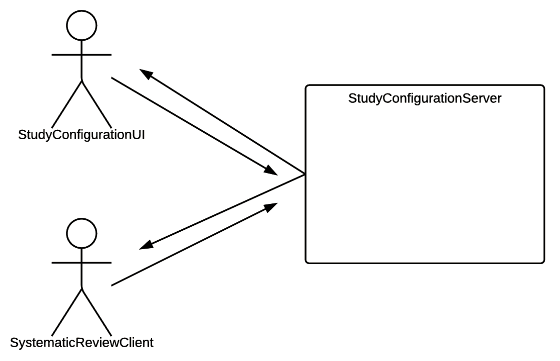
\includegraphics[width=.95\textwidth]{./uml/SysModel.png}
    \caption{System Model for Glitter.}
    \label{fig:SysModel}
\end{figure}


\section{Use Case Models}

\subsection{Scenarios}
\begin{center}
	\begin{tabular}{ | l | p{9cm} |} \hline
	    Scenario name & \textbf{Conducting a review}\\ \hline
	    Participating Actor instances &  Bob: Researcher Alice: Reviewer\\ \hline
	    Flow Of Events &
	    \begin{enumerate}
		   \item Alice just had lunch with Bob, when he told Alice that he had assigned Alice to review a study about waves and how they can produce electricity. Bob wanted Alice to review and screen papers for the study by next week.
		   \item As soon as Alice turns on the program she immediately sees that she has been assigned for screening for the wave study.
		   \item Alice reads up on what the review wants her to do, this time she has to go through a list of 51 articles and look for relevant papers that match the topic of harnessing electricity from waves. The articles she find corresponding with the topic she marks off.
		   \item At 4 pm Alice has a appointment so she shuts down her pc and decides to finish reviewing the last 9 papers tomorrow.
	    \end{enumerate}\\ \hline
	\end{tabular}
\end{center}

\hspace{1.5cm}

\begin{center}
	\begin{tabular}{ | l | p{9cm} |} \hline
	    Scenario name & \textbf{Retrieving papers for screening}\\ \hline
	    Participating Actor instances &  Bob: Researcher, Alice: Researcher\\ \hline
	    Flow Of Events &
	    \begin{enumerate}
		    \item Bob needs to retrieve papers for a seismic analysis article he got yesterday.
		    \item Bob is wondering if there are many people whom wrote on the topic before? He starts searching the system for papers with the topics ?seismic activity? and ?volcanic eruptions?.
		    \item Bob gets a long list of papers shown on the screen, he finds that some of the articles are written by Alice.
		    \item Bob downloads the articles Alice has published after 2011 and are under 6 pages, so he can read them on the way home.
		    
	    \end{enumerate}\\ \hline
	\end{tabular}
\end{center}

\hspace{1.5cm}

\begin{center}
	\begin{tabular}{ | l | p{9cm} |} \hline
	    Scenario name & \textbf{Planning a study}\\ \hline
	    Participating Actor instances &  Bob: Researcher/Study manager\\ \hline
	    Flow Of Events &
	    \begin{enumerate}
		    \item Bob wants to create a new study of a subject, he decides that waves producing electricity could be an intriguing subject.
		    \item Bob creates a new study and enters the research question: ?how can waves produce electricity?, together with some inclusion and exclusion criteria that older papers than 2005 are to old for this study to have any relevance.
		    \item Bob must choose a team to conduct the study. Bob chooses his own team with him and Alice.
		    \item After Bob chose a team he now has to set up the workload and phases of the study, Bob Chooses to have 3 phases and he wants to distribute the work equally among him and Alice.
		    \item Bob is now done with his study planning and can submit his study and begin working.
		    		    
	    \end{enumerate}\\ \hline
	\end{tabular}
\end{center}

\hspace{1.5cm}

\begin{center}
	\begin{tabular}{ | l | p{9cm} |} \hline
	    Scenario name & \textbf{Exporting the data}\\ \hline
	    Participating Actor instances &  Bob: Researcher\\ \hline
	    Flow Of Events &
	    \begin{enumerate}
		    \item Bob and his research team has just finished conducting the review and now they want to report it.
		    \item He decides that they want bubble graphs, bar charts and a couple of tables to illustrate their findings.
		    \item Bob receives the illustrations as figures which he can now use for their report.
		    		    
	    \end{enumerate}\\ \hline
	\end{tabular}
\end{center}
\pagebreak


\subsection{Use Case Model}
\begin{figure}[!h]
    \centering
    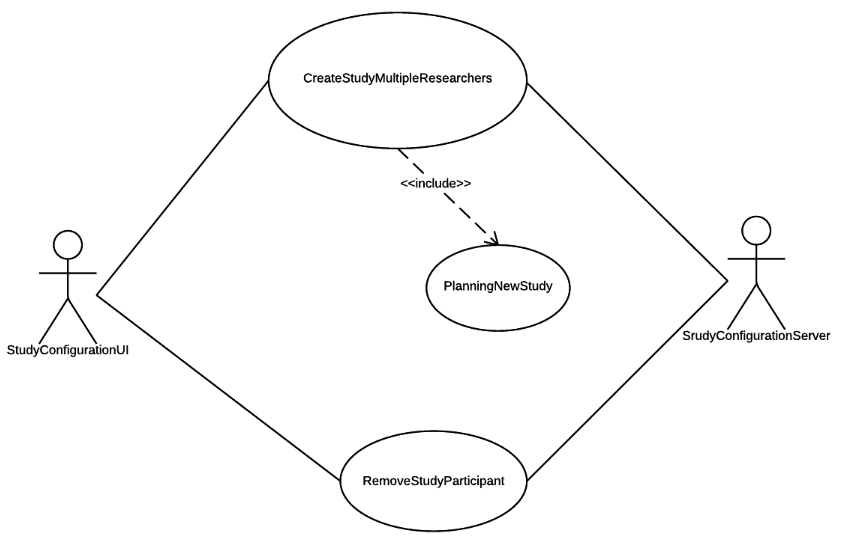
\includegraphics[width=.95\textwidth]{./uml/use_case_model.png}
    \caption{Use Case model for Glitter}
    \label{fig:CreateStudy}
\end{figure}

\subsection{Use Cases}
\begin{center}
	\begin{tabular}{ | l | p{10cm} |} \hline
	    Use Case Name & \textbf{Marking papers off for a study}\\ \hline
	    Participating Actors &  Initiated by reviewer, Communicates via StudyConfigurationUI, StudyConfigurationServer\\ \hline
	    Flow Of Events &
	    \begin{enumerate}
		    \item The reviewer presses the button "See my tasks" in the StudyConfigurationUI.
		    \item StudyConfigurationUI shows an overview of tasks that are assigned to the reviewer.
		    \item The reviewer double-clicks on a specific task to see the details of that task.
		    \item StudyConfigurationUI opens the task, and shows the study plan for this specific task. 
		    \item The reviewer selects to start the review process.
		    \item StudyConfigurationUI retrieves the papers corresponding to the specified criteria of the study from the StudyConfigurationServer and lists the papers on the screen.
		    \item The reviewer reads one paper at the time and marks the ones that are relevant to the study off.
		    \item When done, the reviewer presses "submit" and the papers marked off are stored on the task.
		    \item StudyConfigurationUI prompts if reviewer want to change the task to "Done"
		    \item Reviewer confirms that the task has been done.
	     	    		    	    
	    \end{enumerate}\\ \hline
	    Entry Condition & 
	    \begin{enumerate}
		    \item[-] A task asking to find papers with a given criteria is assigned to the reviewer.
		    \item[-] The Researcher is connected to the internet/System Configuration Server.
	    \end{enumerate}
	    \\ \hline
	    Exit Condition &
	   	\begin{enumerate}
	   		\item[-] The reviewer has successfully submitted a list of papers and changed the status of the task to "done".
	   		\item[-] The reviewer has aborted the reviewing process.
	   	\end{enumerate}
	   	\\ \hline
	    Quality Requirements & No more than 5 seconds should pass before the researcher receives a response after pressing a button.
	    The user should be able to cancel the process of reviewing at any time and still be able to save the progress made.\\ \hline
	\end{tabular}
\end{center}

\begin{center}
	\begin{tabular}{ | l | p{10cm} |} \hline
	    Use Case Name & \textbf{CreateStudyMultipleResearchers}\\ \hline
	    Participating Actors &  Initiated by Researcher, Communicates via StudyConfigurationUI, StudyConfigurationServer\\ \hline
	    Flow Of Events &
	    \begin{enumerate}
		    \item The researcher presses the “Create new study” button in the StudyConfigurationUI.
		    \item The StudyConfigurationUIresponds by asking the researcher for a name and a topic for the study.
		    \item The researcher enters a name and topic and presses “next”.
		    \item The StudyConfigurationUI responds by asking if any other researchers are to be assigned to the study, prompting the researcher with a field for a name, as well as a button saying add.
		    \item The researcher enter the name of a fellow researcher, and presses the “add” button.
		    \item The StudyConfigurationUI verifies the name of the user with the StudyConfigurationServer.
		    \item If the name of the new researcher is present in the StudyConfigurationServer, the researcher is added to the new study.
		    \item Otherwise, the StudyConfigurationUI prompts the researcher that the name of the new researcher could not be verified.
		    \item When the researcher has finished adding all of his coworkers, he presses the “Finish” button, and the study is assigned to the study in the StudyConfigurationServer.
		    		    	    
	    \end{enumerate}\\ \hline
	    Entry Condition & 
	    \begin{enumerate}
		    \item[-] The Researcher wants to create a new study.
		    \item[-] The Researcher is connected to the internet/System Configuration Server.
	    \end{enumerate}
	    \\ \hline
	    Exit Condition &
	   	\begin{enumerate}
	   		\item[-] The researcher has successfully assigned a team to the study.
	   		\item[-] The researcher has aborted the assignment of a team to the study.
	   	\end{enumerate}
	   	\\ \hline
	    Quality Requirements & No more than 10 seconds should pass before the researcher receives a response after pressing “next” “add” or “finish”.
	    The user should be able to cancel the creation of a study at any time.\\ \hline
	\end{tabular}
\end{center}


\begin{center}
	\begin{tabular}{ | l | p{10cm} |} \hline
	    Use Case Name & \textbf{PlanningNewStudy}\\ \hline
	    Participating Actors &  Initiated by Researcher, Communicates via StudyConfigurationUI, StudyConfigurationServer\\ \hline
	    Flow Of Events &
	    \begin{enumerate}
		    \item The researcher enters the criteria he wishes to impose on the study if any into the StudyConfigurationUI and presses “add”.
		    \item The StudyConfigurationUI responds with a messages saying the criteria was added and clears the criteria field so a new criteria can be added.
		    \item The researcher selects the number of phases required for the study, and how the workload should be distributed through each phase, in the StudyConfigurationUI.
		    \item When the researcher is finished selecting phases and workload distribution and has added the desired criteria to his study, he presses “Create study” and the study information is sent via the StudyConfigurationUI to the StudyConfigurationServer.
		    \item The StudyConfigurationUI responds with a message saying the study was created.
		    \item The Study is created on the StudyConfigurationServer.
		    		    		    	    
	    \end{enumerate}\\ \hline
	    Entry Condition & 
	    \begin{enumerate}
		    \item[-] The Researcher wants to create a new study.
		    \item[-] The Researcher has completed the “CreateStudyMultipleResearchers” use case.
		    \item[-] The Researcher is connected to the internet/System Configuration Server.    
	    \end{enumerate}
	    \\ \hline
	    Exit Condition &
	   	\begin{enumerate}
	   		\item[-] The researcher has successfully planned a study.
	   		\item[-] The researcher has aborted planning a study.
	   	\end{enumerate}
	   	\\ \hline
	    Quality Requirements & No more than 10 seconds should pass before the researcher receives a response after pressing a button.
	    The user should be able to cancel the creation of a study at any time.\\ \hline
	\end{tabular}
\end{center}

\begin{center}
	\begin{tabular}{ | l | p{10cm} |} \hline
	    Use Case Name & \textbf{RemoveStudyParticipant}\\ \hline
	    Participating Actors &  Initiated by Researcher with Admin flag, Comminucates via StudyConfigurationUI, StudyConfigurationServer\\ \hline
	    Flow Of Events &
	    \begin{enumerate}
		    \item The researcher presses the “Manage studies” button in the StudyConfigurationUI
		    \item The StudyConfigurationUI responds by presenting the researcher with a list of studies for which he is one of the registered admins.
		    \item The researcher selects the study for which he wants to edit participants, then presses the “Edit” button.
		    \item The StudyConfigurationUI responds by presenting the reasercher with a list of all participants, as well as other options for the study.
		    \item The researcher select the participant he wants to remove from the study, and then presses the “Remove” button.
		    \item When the researcher is finished editing the study, he presses the “Apply” button, followed by the “Exit” button and is returned to the main menu.	    
	    \end{enumerate}\\ \hline
	    Entry Condition & 
	    \begin{enumerate}
		    \item[-] The researcher wants to remove a participant from a study.
		    \item[-] The researcher is connected to the internet/System Configuration Server.
	    \end{enumerate}
	    \\ \hline
	    Exit Condition &
	   	\begin{enumerate}
	   		\item[-] The researcher successfully removed the participant from the study.
	   	\end{enumerate}
	   	\\ \hline
	    Quality Requirements & No more than 10 seconds should pass before the researcher receives a response after pressing “Edit”, “Remove”, “Apply”  or “Exit”.\newline
	    The researcher should be able to revert any changes, up until the point of pressing “apply”\\ \hline
	\end{tabular}
\end{center}

%
%%\usecase{
%%    title = {XXX},
%%    label = uc:xxx,
%%    description = {abc},
%%    scope = {scope},
%%    level = {level},
%%    actors = {Initiated by \emph{XXX}},
%%    stakeholders and interests = {all},
%%%    precondition = { None. },
%%    preconditions = {
%%        \item 1
%%        \item 2
%%        \item 3  
%%    },
%%%    postcondition = {Something.},
%%    postconditions = {
%%        \item 1
%%        \item 2
%%        \item 3
%%    },
%%    main success scenario = {
%%        \item 1
%%        \item 2
%%        \item 3
%%        \item 4
%%    },
%%    extensions = {
%%        \item 1
%%        \item 2
%%        \item 3
%%    },
%%    special requirements = {
%%	    \item 1
%%        \item 2
%%		\\
%%	},
%%    frequency of occurrence = Often,
%%    open issues = {A lot of things...},
%%}
%
%
%%\usecase{
%%    title = View Patient Dashboard,
%%    label = uc:phone_dashboard,
%%    description = {This use case begins when a \emph{Patient} enters the application or requests to see the patient dashboard -- the main screen of the application.},
%%    actors = Initiated by \emph{Patient.},
%%    precondition = { None. },
%%    main success scenario = {
%%        \item The system displays the \glspl{patient_dashboard} with all the content.
%%    },
%%    frequency of occurrence = Often,
%%    frequency of occurrence = Regularly,
%%    frequency of occurrence = Seldom,
%%}
%




%================================================================================================

\section{Domain Object Models}
%
% - Identify nouns in system (potential classes)
% - Identify relationships between nouns (potential associations)
% - Refine class list
% - Identify aggregation relationships
% - Identify inheritance relationships
% - Iterate
%

%================================================================================================

\section{Dynamic Models}
%
% The next subsection contains the diagrams describing behavior, including
% the state diagrams and sequence diagrams
% - Create a state diagram for entire system
% - Use use cases to provide scenarios of events in system
% - Create sequence diagrams for scenarios capturing messages between objects;
%   include sequence diagrams for normal and special case usage scenarios
% - Create state diagrams to capture behavior of objects 
% - Iterate and refine state diagrams


\subsection{Use Case Sequence Diagrams}


\subsection{State Diagrams}


%================================================================================================
\section{User Interfaces}
%Navigational paths and screen mock-ups



\subsection{Graphical User Interface for Operator}




\part{Software Design Document}
\label{part:sdd}

\chapter{Current Software Architecture}
\label{sec:current_architecture}







\chapter{Proposed Software Architecture}
\label{sec:proposed_architecture}
\section{Design Goals}

%Overview presents a bird?s-eye view of the software architecture and briefly describes the assignment of functionality to each subsystem.
\section{Overview}

% Subsystem decomposition describes the decomposition into subsystems and the responsibilities of each. This is the main product of system design.
\section{Subsystem Decomposition}
\label{sec:subsystems}


%Persistent data management describes the persistent data stored by the system and the data management infrastructure required for it. This section typically includes the description of data schemes, the selection of a database, and the description of the encapsulation of the database.
\section{Persistent Data Management}

% Access control and security describes the user model of the system in terms of an access matrix. This section also describes security issues, such as the selection of an authentication mechanism, the use of encryption, and the management of keys.
\section{Access Control and Security}

%Global software control describes how the global software control is implemented. In particular, this section should describe how requests are initiated and how subsystems synchronize. This section should list and address synchronization and concurrency issues.
\section{Global Software Control}

%Boundary conditions describes the start-up, shutdown, and error behavior of the system. (If new use cases are discovered for system administration, these should be included in the requirements analysis document, not in this section.)
\section{Boundary Conditions}




\part{Object Design Document}
\label{part:odd}

\chapter{Object Design and Patterns}
\label{sec:object_design}

%Detailed description of (final) object design, i.e. the class diagram.
\section{Object Design}

\section{Interfaces}

\section{Design Patterns}



\part{Test Document}
\label{part:test}

\chapter{Test Plan and Results}
\label{sec:test}


\section{Overall Test Approach}

\section{Component / Unit Testing}

\section{Integration Testing}

\section{System Testing}

%\section{Acceptance Testing}








%\part{SCRUM Documentation}

%\chapter{SCRUM}
%\label{sec:scrum}
%
% This section describes how you organized the SCRUM process, including who played the different scrum roles, what tools you used, and how you organized the different scrum activities. 
\section{SCRUM Organization}

% This section describes you overall backlog and how is was organized into sprints. Include capacity calculations for each sprint
\section{Sprints}

% This section should show the burndown charts for each sprint, and the overall release/project burndown chart.
\section{Burndown Charts}

% This section should contain the main findings from the review and retrospective meetings.
\section{Review and Retrospective}








\appendix


%\bibliographystyle{plainnat}

% The final section contains the sources of any and all references to other
% group documents, articles, books, etc.  that you used in creating this
% document.  You need to have created the file analysis.bib with
% entries for all of your sources.
%
\bibliographystyle{plain}
\bibliography{../../itss} % itss.bib is the bibliography file name

% WHY IS THE BIBLIOGRAPHY NOT IN THE TABLE OF CONTENT?????

% Glossary chapter
% Generated based on glossary entries in ./glossary.tex
\printglossary

\end{document}